\documentclass[11pt]{article}

\usepackage[utf8]{inputenc}
\usepackage[margin=2cm]{geometry} 
\usepackage{hyperref}
\usepackage{graphicx}
\usepackage{float}
\usepackage{caption}
\usepackage{longtable}
\usepackage{minted}
\usepackage{appendix}
\usepackage{xcolor}
\usepackage{subfig}
\usepackage{bookmark}
\usepackage{array}
\usepackage{multirow}
\usepackage{rotating}
\usepackage{placeins}
\usepackage{booktabs}
\usepackage{cite}

\setlength{\parskip}{1em}
\setlength{\parindent}{0pt}

\begin{document}

% ============ TITLE PAGE ============
\title{\huge Data Mining \& Machine Learning F20DL} 
% \\ {\small{\url{ }}}}
\author{Group 4\\Lewis Wilson, Sam Fay-Hunt, Kamil Szymczak, Chun Man }
\date{\today}
\maketitle

% ============ TABLE OF CONTENTS ============
\newpage
\tableofcontents
\thispagestyle{empty}
\pagebreak
\setcounter{page}{1}
% ============ INTRODUCTION ============
\newpage
\section{Introduction}
For both decision trees and neural networks, we used Weights and Biases (\url{https://wandb.ai/home}) to visualise these experiments which we used to record and organise the experiment data shown the graphs shown in this document.



\newpage
\section{Variation in performance with size of the training and testing sets}
\subsection{Methodology}
We used the same seed when moving the data from the training set to the testing set, so all experiments for a given classifier used the same training and testing data.
\subsection{Turn left deep dive}
The turn left dataset has an extremely small number of instances in its training dataset for 9000 moved to testing, Thus we would expect the worst prediction accuracy, in this case, the situation was so bad that our accuracy scores became misleading. Because the representation of ‘turn left’ was so poor in our dataset most of the classifiers simply predicted that there were no instances of turn left in the dataset and recorded a deceiving 97\% accuracy (because 97\% of the dataset is not in fact turn left). In fact this problem appeared for all binary classifications with the Random Forest classifier.
The only classifiers that did not exhibit this behaviour were the Logistic Regression (LR) and Convolutional Neural Network classifiers (CNN). CNN scored a staggering 99.9\% accuracy with the same minuscule training data, while LR managed 98.3\% with 200 false negatives, 5 false positives and 60 true positives.
\newline
\par
\begin{figure}[h]
  \caption {Class proportions in target variable}
  \centering 
  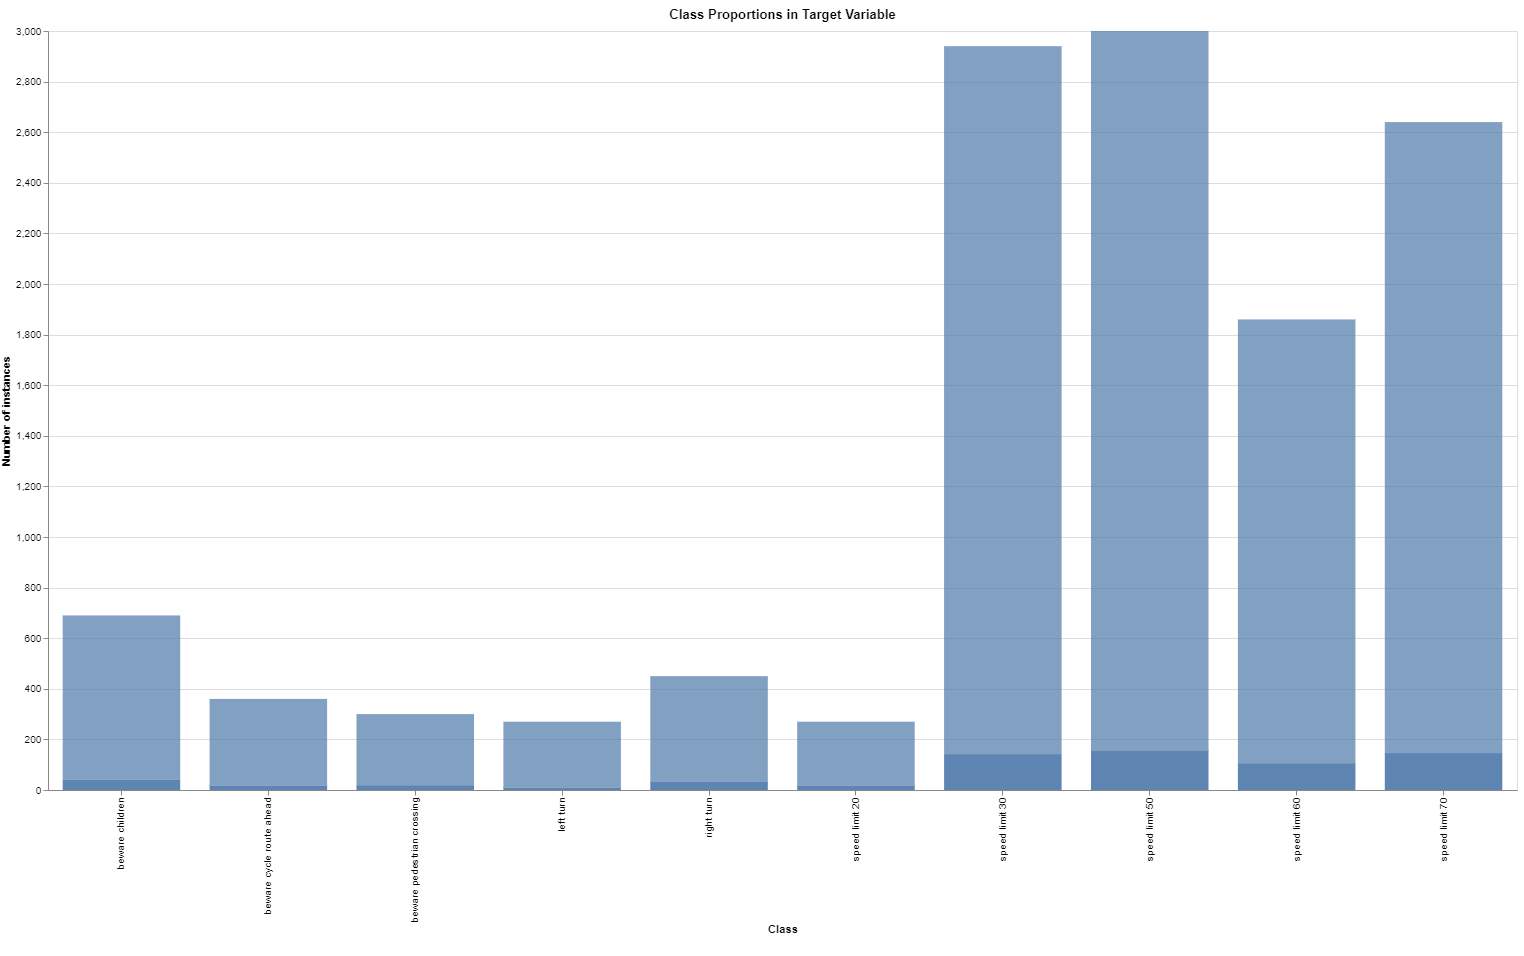
\includegraphics[width = \textwidth, height = 0.5\textheight, keepaspectratio]{Images/classProportionsInTargetVariable.png}
\end{figure}
An example distribution of labels between train (dark blue) and test (light blue), for the Beware cycle route ahead class. 

\newpage
\subsection{Original train \& test sets}
\begin{figure}[h]
  \caption {Class proportions in target variable}
  \centering 
  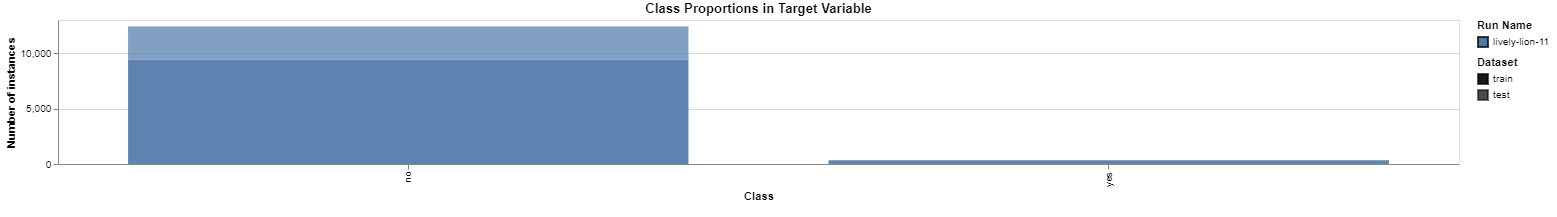
\includegraphics[width = \textwidth, height = 0.5\textheight, keepaspectratio]{Images/Sec1Original.png}
\end{figure}

\subsection{4000 moved}
\begin{figure}[h]
  \caption {Class proportions in target variable}
  \centering 
  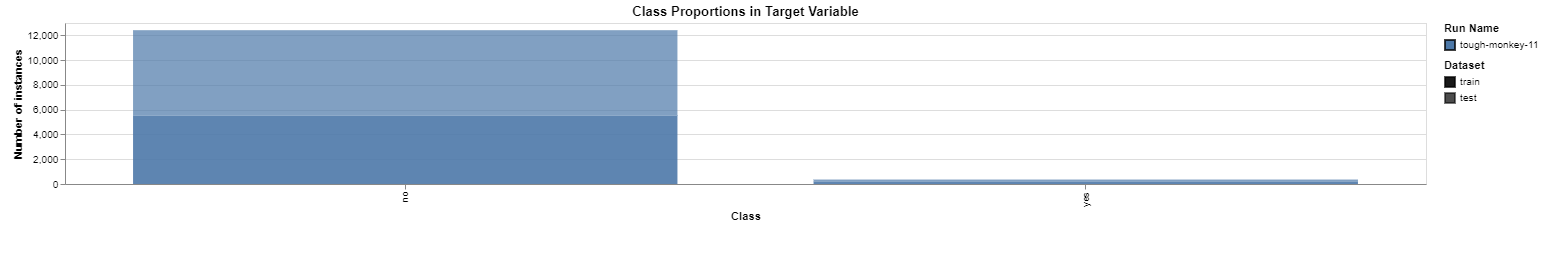
\includegraphics[width = \textwidth, height = 0.5\textheight, keepaspectratio]{Images/Sec1-4k.png}
\end{figure}

\subsection{9000 moved}
\begin{figure}[h]
  \caption {Class proportions in target variable}
  \centering 
  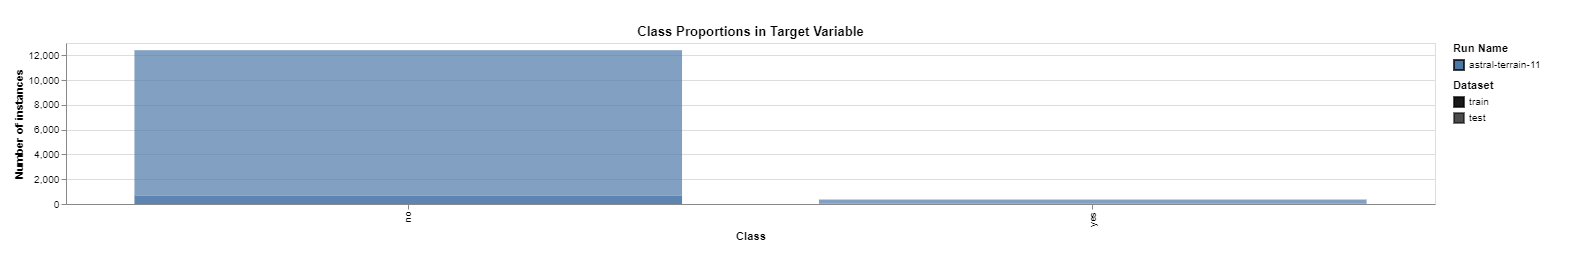
\includegraphics[width = \textwidth, height = 0.5\textheight, keepaspectratio]{Images/Sec1-9k.png}
\end{figure}


Starting out we observed the results of J48, the issues are immediately clear, even in the experiment with the full training set J48 is poor at attempting to predict on this kind of data, when working with all classes it is unable to reliably distinguish between the different speed limit signs, and the other signs consistently are quite evenly classified with any class label.

\begin{figure}[h]
  \caption {J48 Confusion Matrix}
  \centering 
  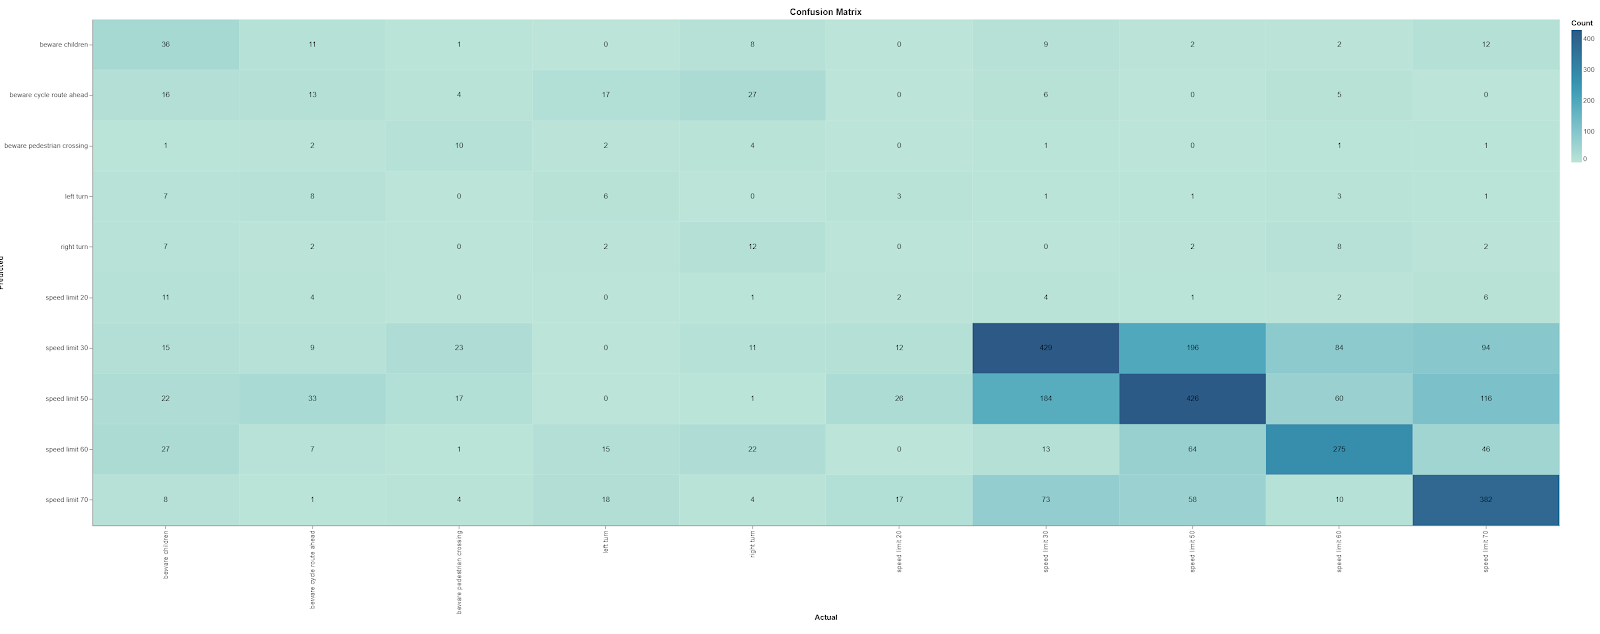
\includegraphics[width = \textwidth, height = 0.3\textheight, keepaspectratio]{Images/J48ConfMat.png}
\end{figure}
\FloatBarrier
As the test set grows we can observe a similar story, however the classifier gets substantially worse at distinguishing between speed limit signs and other signs because the representation of those signs in the dataset gets very low.

With all the classifiers except Logistic Regression we see the same story, Multi-layer perceptron and random forest particularly suffers from this poor class representation issue in the data. We can see for figure [x] that the Multilayer perceptron assigns most labels for 3 classes: Speed limit 30, 50, 70. It also assigns a small number of labels for speed limit 70.


\begin{figure}[h]
  \caption {Multilayer Perceptron Confusion Matrix}
  \centering 
  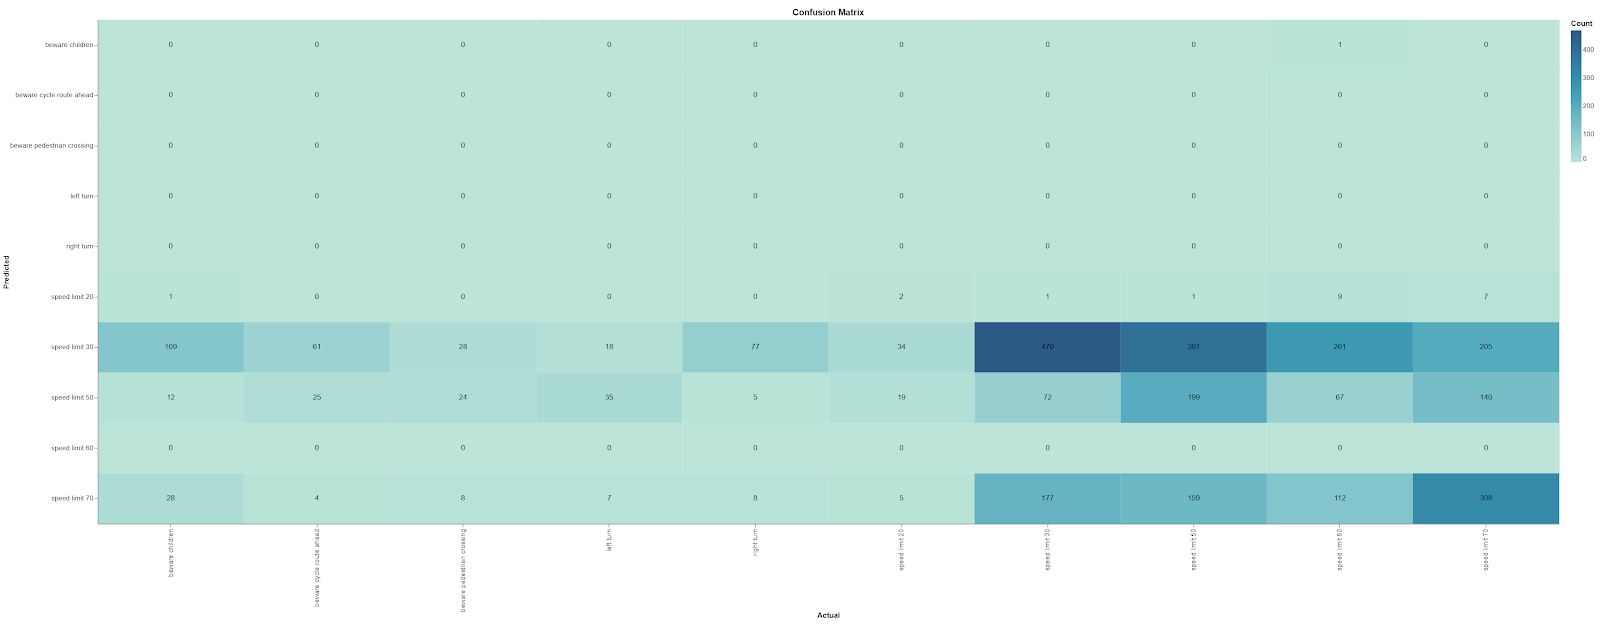
\includegraphics[width = \textwidth, height = 0.3\textheight, keepaspectratio]{Images/Sec1-ConfMat2.png}
\end{figure}

\newpage
\section{Variation in performance with the change in the learning paradigm (Decision Trees versus
Neural Nets)}
\begin{itemize}
  \item Decision trees performed comparatively poorly, particularly when the training data was reduced.
  \item Multilayer Perceptron had overfitting issues, Logistic Regression was the best, aside from the CNN
\end{itemize}
We have found decision trees performed very poorly particularly when the training data was reduced and also so did the MultiLayer Perceptron which had overfitting issues. Both of these classifiers had 0 recall and 0 precision for predicting individual classes datasets. This means they have not predicted correctly a single sign and should not be used in prediction road signs from images. Our results perfectly support the weak points about decision trees such as that there are variable relationships that decision trees just can’t learn and they are unstable as a small change in the data can lead to a large change in the structure of the optimal decision tree \cite{zhaoComparisonDecisionTree2008}.
\par
However Logistic Regression performed considerably better, it was actually the best performer from all classification techniques we have used and tested, aside from the CNN. 
\par
Logistic Regression gives the best results because the benefit of logistic regression is its interpretability as it understands which pixels are important to determine what class an image belongs to.
\par
Convolutional Neural Networks worked phenomenally as expected, as they are widely used in image classification.


\newpage
\section{Variation in performance with varying learning parameters in Decision Trees}
% ===================================== J48 =====================================
\subsection{Optimising Hyperparameters}

Our hyperparameter optimization used Bayesian Optimization \cite{Configuration}. This gaussian process models the function and then chooses parameters to optimize by determining the probability of improvement according to the accuracy metric. 
\par
We opted to use the ‘all classes’ dataset for these sweeps because in our preliminary experiments we noticed the worst prediction accuracy with 10 classes.

Figure below shows high level overview of the MLP sweep, dark blue lines indicate lower accuracy and yellow had the highest accuracy. (See \ref{MLPSection})

\begin{center}
  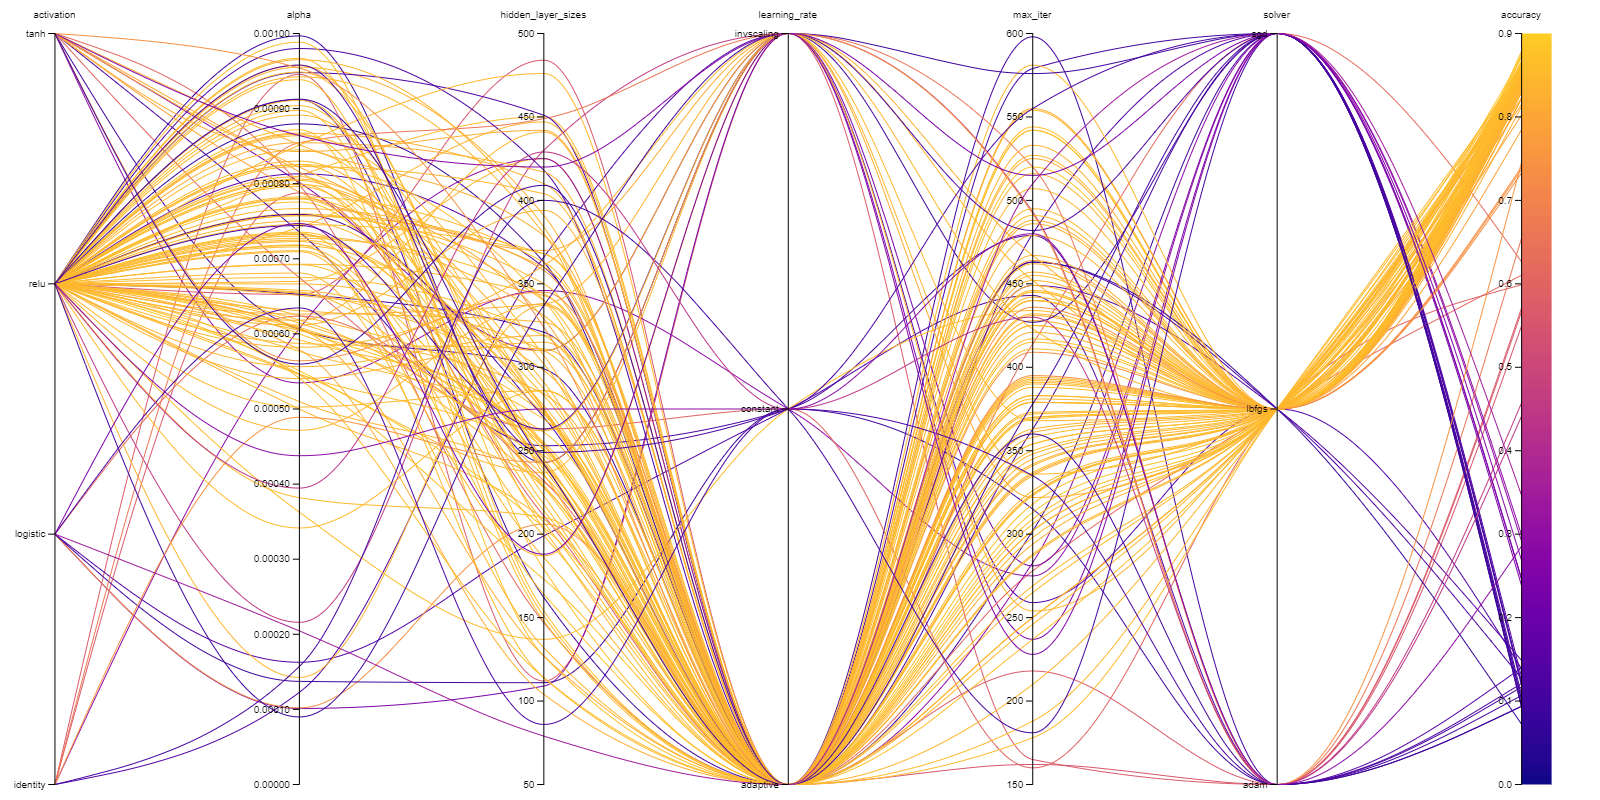
\includegraphics [width = \textwidth, height = 0.3\textheight, keepaspectratio]{Images/MLP ParallelCoordGraph.png}
\end{center}

\textcolor{red}{\textbf{To evaluate the hyperparameters we collected and evaluated the linear correlation between the hyperparameter and the accuracy, and also a feature importance metric provided by weights and biases, this metric is computed by training a random forest with the hyperparameters as inputs and the accuracy as the target output, the feature importances are then extracted from the random forest. \url{https://docs.wandb.com/app/features/panels/parameter-importance}
}}
\par
The feature importance metric is useful to identify the features that have a larger impact on the output of the model, coupled with correlation we can find the direction of the relationship. It may be the case that a very important feature is extremely bad for the result, in this case we will see a strong negative correlation, this information helps us hone in on the best hyperparameters to use to maximise accuracy.
\par
This however caused the models to instead maximise hyperparameters tendency to overfit this very imbalanced dataset.
\newpage
\subsection{J48}

Discussed below is the hyperparameter \cite{SklearnTreeDecisionTreeClassifier} importance concerning the performance of J48 trees:

\textbf{max\_depth -} The maximum depth of the tree. \\
\textbf{min\_impurity\_decrease -} Splits a node if this split induces a decrease of the impurity greater than or equal to this value. \\
\textbf{min\_samples\_leaf -} the minimum number of samples to be considered a leaf. \\
\textbf{min\_weight\_fraction\_leaf -} The minimum number of samples required to be at a leaf node. \\
\textbf{criterion\_value -}[‘Gini’,’Entropy’]: Measures the quality of the split.
\textbf{max\_features -} [‘auto’,’log2’,’sqrt’] : max features considers the number of features when looking for the best split. Auto just picks the best result so had the same result as log2. \\
\textbf{Splitter -} [‘best’, ‘random’]: The strategy used to choose the split at each node. 
\newline

\begin{table}[h]
  \centering
  \begin{tabular}{|p{0.25\linewidth} | p{0.15 \linewidth} | p{0.45\linewidth}|} 
    \hline
    \textbf{Parameter}  & \textbf{Type} &\textbf{Conclusion} \\ \hline
    max\_depth & int & Provided low importance value of 0.012 and provided some correlation 0.084. \\ \hline
    min\_impurity\_decrease & float & Small importance value of 0.051 and a strong negative correlation of -0.241.  \\ \hline
    min\_samples\_leaf & int or float & Low importance of 0.014 and provided a tiny positive correlation of 0.007. \\ \hline
    min\_weight\_fraction\_leaf & float & Gives a strong negative correlation in terms of accuracy, meaning the higher the min\_weight\_fraction\_leaf value, the lower the accuracy.\\ \hline
    criterion & string & Both parameters provided a very low importance value of 0.003. Entropy had a tiny negative correlation of -0.022 and Gini a positive correlation of 0.022. \\ \hline
    max\_features & string & Log2 provided an importance value of 0.133 and a high negative correlation of -0.372. Log2 provided tiny importance of 0.003 but a relatively good correlation of 0.196. \\ \hline
    splitter & string & 'best' had an importance of 0.048 and random 0.044. 'best' has a positive correlation of 0.051 whereas random -0.051. \\ \hline
  \end{tabular}
\end{table}\label{RF_Analysis_Table}
See Parameter Importance (Figure \ref{J48_ParamImp1})
\FloatBarrier
% ===================================== RANDOM FOREST =====================================

\newpage
\subsection{Random Forest}
\textbf{min\_samples\_split -} The minimum number of samples required to split an internal node \\
\textbf{min\_samples\_leaf -} The minimum number of samples required to be at a leaf node.  \\
\textbf{n\_estimators -} The number of trees in the forest.\\
\textbf{min\_weight\_fraction\_leaf -} The minimum number of samples required to be at a leaf node. \\
\textbf{max\_features -} The number of features to consider when looking for the best \\
\textbf{criterion -} The function to measure the quality of a split. Supported criteria are “gini” for the Gini impurity and “entropy” for the information gain. \\


\begin{table}[ht]
  \centering
  \begin{tabular}{|p{0.25\linewidth} | p{0.15 \linewidth} | p{0.45\linewidth}|} 
    \hline
    \textbf{Parameter}  & \textbf{Type} & \textbf{Conclusion} \\ \hline
    max\_features & string & Contains the options "auto", "sqrt" and "log2". We discovered that "sqrt" has a higher accuracy overall, the accuracy of "log2" varies between the lower end and the median accuracy value.\\ \hline
    min\_samples\_split & int or float & The minimum samples required to split a node has very little impact on accuracy.  \\ \hline
    criterion & string & Gives a perfect negative correlation with respect to accuracy. Correlation values being [Gini = -0.404 ], [Entropy = 0.404 ]. \\ \hline
    n\_estimators & int & This is defined as the number of trees in the forest, it seems to have very little correlation but high importance. \\ \hline
    min\_samples\_leaf & int or float & Gives a strong negative correlation in terms of accuracy, meaning the higher minimum samples at a leaf node, the lower the accuracy. \\ \hline
    min\_weight\_fraction\_leaf & float & Has a somewhat positive correlation to accuracy. e.g. total weight required at a leaf node varies between 76\% and 89\% accuracy\\ \hline
  \end{tabular}
\end{table}\label{RF_Analysis_Table}
See Parameter Importance (Figure \ref{RF_ParamImp1})

\newpage
\section{Variation in performance with varying learning parameters in Neural Networks}
% ===================================== LINEAR CLASSIFIER =====================================
\subsection{Linear Classifier}

For a linear classifier we have decided to use logistic regression. 
Shown below is the hyperparameter importance concerning the performance of Logistic Regression.

The accuracy fluctuates depending on which hyperparameters are used. Logistic Regression has a ‘solver’ hyperparameter in sklearn which is the algorithm to use in the optimization. We have tested the following: ‘newton-cg’, ‘lbfgs’, ‘liblinear’, ‘sag’, ‘saga’. Sag and Saga give the best results with 89\% accuracy. Liblinear isn't far behind with 88%.
Other solvers have a negative impact on the performance, this can be seen in the Solver parameter importance table where their correlation values are negative.

Additionally ‘sag’ and ‘saga’ guarantee fast convergence on features with approximately the same scale [R41] which is the case with our datasets as pixel values have the same scale. This can be seen as the number of iterations between 200-800 don’t change much in the accuracy and from the scatter chart of the accuracy of the Logistic Regression vs the number of sweeps created.

\begin{table}[ht]
  \centering
  \begin{tabular}{|p{0.25\linewidth} | p{0.15 \linewidth} | p{0.45\linewidth}|} 
    \hline
    \textbf{Parameter} & \textbf{Type} & \textbf{Conclusion} \\ \hline
    C & float & The smaller this value is the stronger the regularization. For this we settled on 0.08027. Although this parameter did not make a big d ifference and provided similar results for values between 0.8 and 1.2 \\ \hline
    fit\_intercept & bool & From testing we have found out that for this dataset adding a bias works better than not having bias thus True  \\ \hline
    max\_iter & int &  We settled on 342 maximum number of iterations taken for the solver to converge. This parameter does not have a big importance but we found 342 gives accurate results. \\ \hline
    solver & string & Contains the options ‘newton-cg’, ‘lbfgs’, ‘liblinear’, ‘sag’, ‘saga’, default=’lbfgs’. ‘Saga’ gives the best accuracy overall. Solver is the most influential hyperparameter as we can see from the importance and correlation table \\ \hline
    tol & float & tolerance for stopping criteria which tells the algorithm to stop searching when some tolerance is achieved. This parameter did not make a difference, we settled on 0.0002277 \\ \hline


  \end{tabular}
\end{table}\label{RF_Analysis_Table}
See Parameter Importance (Figure \ref{LC_ParamImp1})

% ===================================== MULTILAYER PERCEPTRON =====================================
\newpage
\subsection{Multilayer Perceptron}
\label{MLPSection}
\textcolor{red}{ADD PARAM DEFINITIONS}
\begin{table}[ht]
  \centering
  \begin{tabular}{|p{0.25\linewidth} | p{0.15 \linewidth} | p{0.45\linewidth}|} 
    \hline
    \textbf{Parameter} & \textbf{Type} & \textbf{Conclusion} \\ \hline
    alpha & float & This has a positive correlation to accuracy as higher alpha value equates to higher accuracy. \\ \hline 
    solver & string & ‘Lbfgs’ solver did provide the best accuracy consistently when compared to other solvers such as ‘adam’ and ‘sgd’ which supports the statement from [X002] staying that ‘Lbfgs’ works best for small datasets. \\ \hline
    max\_iter & int & The maximum number of iterations - In general, higher accuracy can be achieved with a larger amount of max iterations. \\ \hline
    activation & string & Out of the four activation functions (relu, tanh, identity and logistic), relu is the only one with a positive correlation, giving the highest accuracy overall. \\ \hline  
    learning\_rate & string & 'adaptive' achieves the highest accuracy while, 'constant' and 'invscaling' vary widely. \\ \hline  
    hidden\_layer\_sizes & tuple & Has a negative correlation - the number neurons in the n-th hidden layer has no effect on accuracy. \\ \hline
  \end{tabular}
\end{table}\label{MLP_Analysis_Table}
\FloatBarrier
See Parameter Importance (Figure \ref{MLP_ParamImp1})

% ===================================== CONVOLUTIONAL NEURAL NETWORKS =====================================


\newpage
\subsection{Convolutional Neural Networks}
\begin{center}
  

\begin{table}[h]
  \begin{tabular}{@{}lll@{}}
  \toprule
  Layer type & Output Shape & Param \# \\ \midrule
  conv2D & (None, 48, 48, 75) & 750 \\ \midrule
  BatchNormalization & (None, 48, 48, 75) & 300 \\ \midrule
  MaxPooling2D & (None, 24, 24, 75) & 0 \\ \midrule
  Conv2D & (None, 24, 24, 50) & 33800 \\ \midrule
  Dropout & (None, 24, 24, 50) & 0 \\ \midrule
  BatchNormalization & (None, 24, 24, 50) & 200 \\ \midrule
  MaxPooling2D & (None, 12, 12, 50) & 0 \\ \midrule
  Conv2D & (None, 12, 12, 25) & 11275 \\ \midrule
  BatchNormalization & (None, 12, 12, 25) & 100 \\ \midrule
  MaxPooling2D & (None, 6, 6, 25) & 0 \\ \midrule
  Flatten & (None, 900) & 0 \\ \midrule
  Dense & (None, 512) & 461312 \\ \midrule
  Dense & (None, 512) & 262656 \\ \midrule
  Dropout & (None, 512) & 0 \\ \midrule
  Dense & (None, 10) & 5130 \\ \bottomrule
  \end{tabular}
  \end{table}
 \end{center} 
\subsubsection{Critical limitation of CNN experimental methodology:}
We were unable to disable memoization between experiments over each loop, so all the parameters are restored between runs within a given experiment, consequently we noted only significant changes to the loss when training on all classes, after which convergence was achieved in a single epoch. We attempted to clear the model parameters, clear the GPU memory, and model save the randomly initialised parameters and load them back in between experiments but could not prevent the CNN model using data encoded from previous experiments. This does invalidate our results, when compared to the discrete experiments in the previous sections, however this can be a demonstrable advantage of a CNN, in this situation it consistently correctly classifies the images despite changing the dimensions of the output layer and the classification targets (albeit on the same dataset).


During all experiments with training and testing data, at worst our CNN scored an accuracy of 97\% on the test dataset when classifying all classes, the CNN was capable of correct classification even when 9000 instances were moved from the training set to the testing set.

The CNN was unsurprisingly the best performing classifier, In many of the kfold experiments the CNN managed an accuracy of 100\%, but this could be due in part to the memoization effect between experiments, this is particularly noticeable on the kfold experiments.


\newpage
\section{Variation in performance according to different metrics (TP Rate, FP Rate, Precision,
Recall, F Measure, ROC Area)}
\subsection{J48 Experiments}

J48 with default test set cycle route ahead binary classification gave a very high precision (~0.95) and a really low recall (0.2) 
Precision shows the ratio of true positives to all the positives, therefore in our use case we have a ratio of signs that the classifier classified correctly to the total the classifier thought are positive. 
\par
Using cycle route ahead dataset as an example, for all signs that are actually cycle route ahead signs the recall tells us how many the classifier classified as cycle route ahead  signs. 
Therefore J48 is very picky and doesn't think many signs are cycle route ahead signs. Pretty much all signs it thinks are cycle route ahead signs are indeed cycle route ahead signs. However it also misses a lot of cycle route ahead signs, because it is very picky.
\par
With the default test set, J48 provides a precision, recall and f1 scores of 0 for the right turn, left turn, beware pedestrian crossing and speed limit 20 classes the reason is due to 0 true positive classifications.When we investigate why this is for the beware pedestrian crossing class, we noticed the data has a heavy skew of class proportions towards ‘No’ with very few instances of ‘Yes’ found. In fact, this is the case for all of the class labels with scores of 0 for precision, recall and f1.



% ============ APPENDICES BEGINNING ============================================
\pagebreak
\appendix
\appendixpage
\addappheadtotoc
\begin{appendices}

\section{Appendix A}

% =================== Workload Split Table ===================

\subsection{Workload split}
  
  \begin{table}[ht]
    \centering
    \begin{tabular}{|p{0.2\linewidth} | p{0.75\linewidth}|} 
      \hline
      \textbf{Team member}  & \textbf{Involvement} \\ \hline
      Lewis Wilson & text here \\ \hline
      Chun Man & Contributed to the experimenting and analysis of Random Forest, Report writing. \\ \hline
      Sam Fay-Hunt & text here \\ \hline
      Kamil Szymczak & text here \\ \hline
    \end{tabular}
  \end{table}\label{ContributionTab}

As a team we are happy with everyone's contributions to the project. All team members were punctual and showed up to all scheduled meetings. Sam took the lead as project manager throughout the project delegating the workload and providing support to others.


% =================== J48 APPENDIX here ===================
\newpage
\section{J48}

\subsection{J48 Parameter Importance}
  \begin{table}[ht]
    \centering
    \begin{tabular}{|p{0.3\linewidth} | p{0.3\linewidth}| p{0.3\linewidth}|} 
      \hline
      \textbf{Parameter Config}  & \textbf{Importance} & \textbf{Correlation} \\ \hline
        min\_weight\_fraction\_leaf & 0.668  & -0.666 \\ \hline
        min\_impurity\_decrease & 0.052 & -0.241 \\ \hline
        min\_samples\_leaf & 0.016 & 0.007 \\ \hline
        max\_depth & 0.012 & 0.084 \\ \hline
        min\_samples\_split & 0.009 & -0.108 \\ \hline

    \end{tabular}
  \end{table}\label{J48_ParamImp1}

  \begin{table}[ht]
    \centering
    \begin{tabular}{|p{0.3\linewidth} | p{0.3\linewidth}| p{0.3\linewidth}|} 
      \hline
      \textbf{Parameter Config}  & \textbf{Importance} & \textbf{Correlation} \\ \hline
        max\_features.value\_log2 & 0.133 & -0.372 \\ \hline
        max\_features.value\_sqrt & 0.003 & 0.196 \\ \hline
        splitter.value\_best & 0.049 & 0.051 \\ \hline
        splitter.value\_random & 0.043 & -0.051 \\ \hline
        criterion.value\_entropy & 0.002 & -0.022 \\ \hline
        criterion.value\_gini & 0.002 & 0.022 \\ \hline

    \end{tabular}
  \end{table}\label{J48_ParamImp2}

\begin{figure}[h]
  \caption {J48 Parameters} \label{ParallelCoordJ48}
  \centering 
  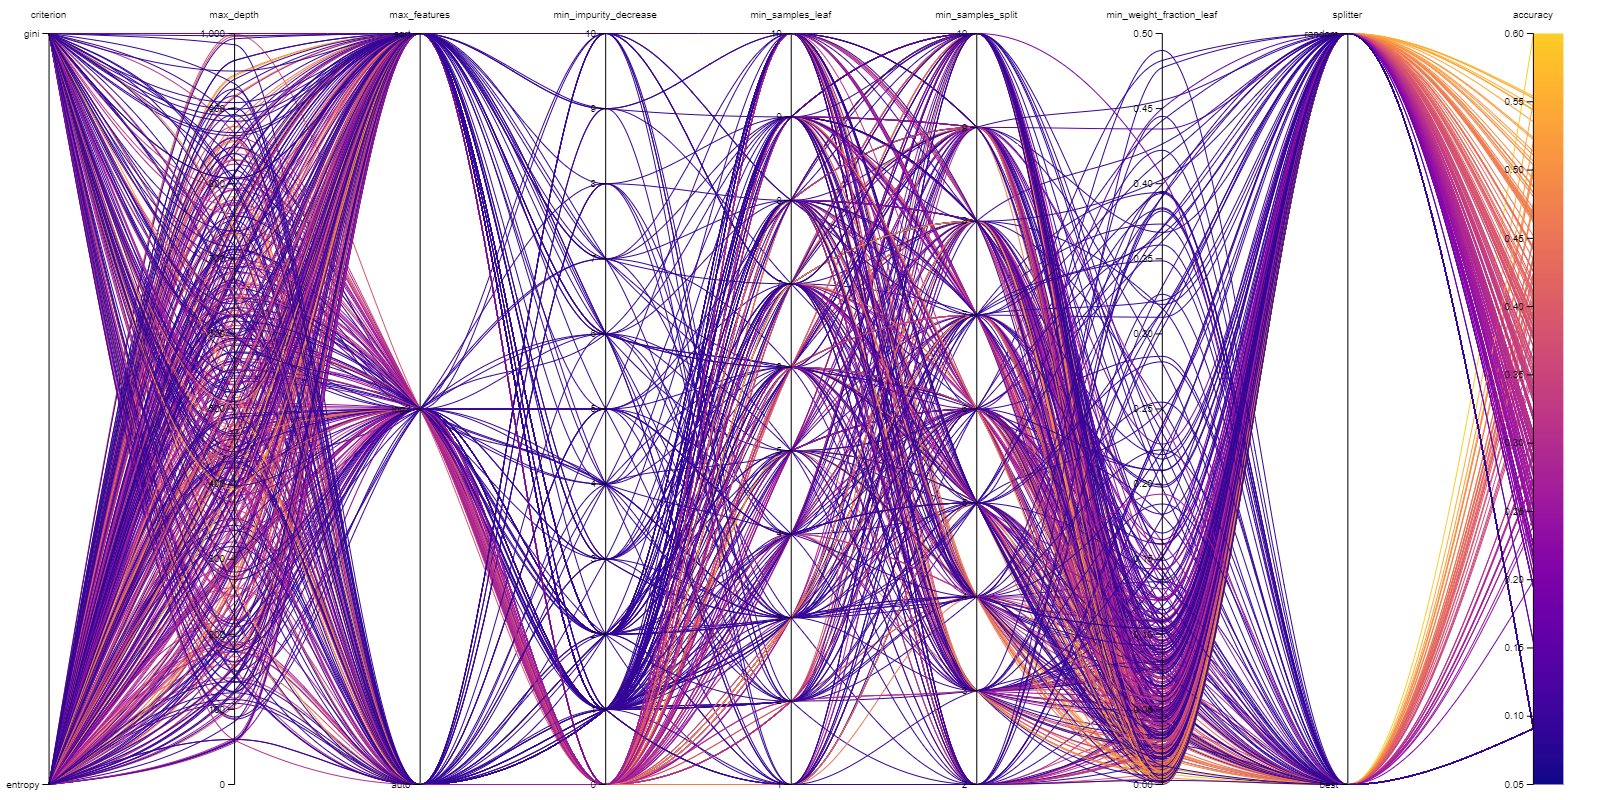
\includegraphics[width = \textwidth, height = \textwidth, keepaspectratio]{Images/J48 ParallelCoordGraph.png}
\end{figure}



\FloatBarrier
% =================== Random Forest APPENDIX here ===================
\newpage
\section{Random Forest}

\subsection{Random Forest Parameter Importance}
  \begin{table}[ht]
    \centering
    \begin{tabular}{|p{0.3\linewidth} | p{0.3\linewidth}| p{0.3\linewidth}|} 
      \hline
      \textbf{Parameter Config}  & \textbf{Importance} & \textbf{Correlation} \\ \hline
        min\_samples\_split & 0.005 & 0.306 \\ \hline
        min\_samples\_leaf & 0.375 & -0.725 \\ \hline
        n\_estimators & 0.016 & 0.092 \\ \hline
        min\_weight\_fraction\_leaf & 0.013 & 0.123 \\ \hline
    \end{tabular}
  \end{table}\label{RF_ParamImp1}

  \begin{table}[ht]
    \centering
    \begin{tabular}{|p{0.3\linewidth} | p{0.3\linewidth}| p{0.3\linewidth}|} 
      \hline
      \textbf{Parameter Config}  & \textbf{Importance} & \textbf{Correlation} \\ \hline
      max\_features.value\_sqrt & 0.001 & 0.563 \\ \hline
      max\_features.value\_log2 & 0.565 & -0.752 \\ \hline
      criterion.value\_entropy & 0.012 & 0.404 \\ \hline
      criterion.value\_gini & 0.012 & -0.404 \\ \hline
    \end{tabular}
  \end{table}\label{RF_ParamImp2}

\begin{figure}[h]
    \caption {Random Forest Parameters} \label{ParallelCoordRF}
    \centering 
    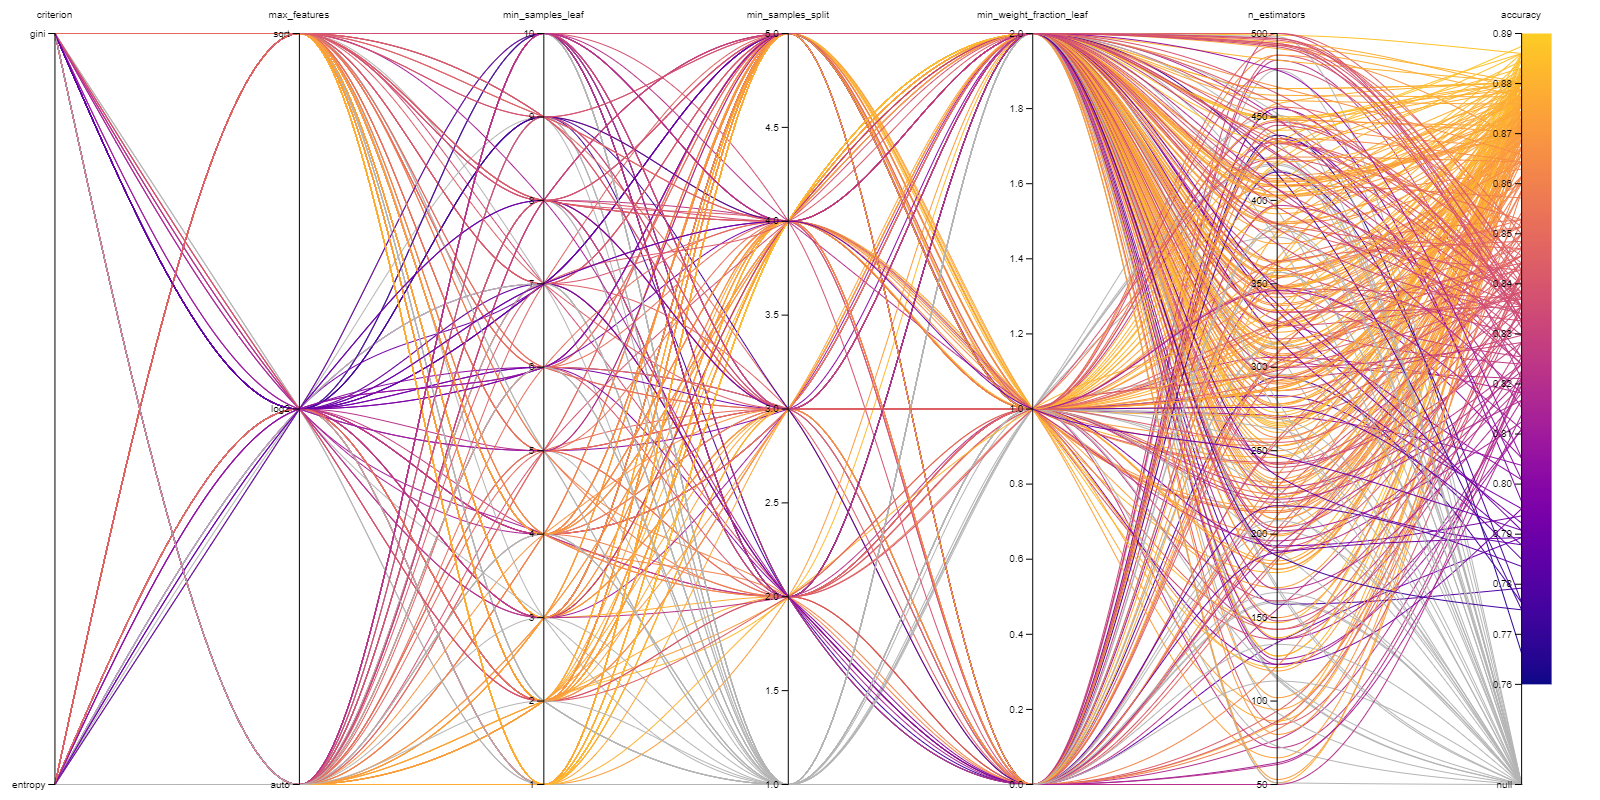
\includegraphics[width = \textwidth, height = \textwidth, keepaspectratio]{Images/RF ParallelCoordGraph.png}
\end{figure}


  
  \FloatBarrier
% =================== Linear Classifier APPENDIX here ===================
\newpage
\section{Linear Classifier}

\subsection{Linear Classifier Parameter Importance}
  \begin{table}[ht]
    \centering
    \begin{tabular}{|p{0.3\linewidth} | p{0.3\linewidth}| p{0.3\linewidth}|} 
      \hline
      \textbf{Solver Parameter Config}  & \textbf{Importance} & \textbf{Correlation} \\ \hline
      lbfgs & 0.786 & -0.869 \\ \hline
      newton-cg & 0.159 & -0.271 \\ \hline
      liblinear & 0.042 & -0.037 \\ \hline
      saga & 0.009 & 0.691 \\ \hline
      sag & 0.003 & 0.170 \\ \hline
    \end{tabular}
  \end{table}\label{LC_ParamImp1}

  \begin{table}[ht]
    \centering
    \begin{tabular}{|p{0.3\linewidth} | p{0.3\linewidth}| p{0.3\linewidth}|} 
      \hline
      \textbf{Config Parameter Config}  & \textbf{Importance} & \textbf{Correlation} \\ \hline
      max-iter & 0.194 & -0.634 \\ \hline
      l1-ratio & 0.124 & -0.510 \\ \hline
      fit-intercept & 0.058 & 0.367 \\ \hline
      tol & 0.046 & -0.174 \\ \hline
      C & 0.031 & 0.260 \\ \hline
    \end{tabular}
  \end{table}\label{LC_ParamImp2}

\begin{figure}[h]
    \caption {Random Forest Parameters} \label{ParallelCoordLC}
    \centering 
    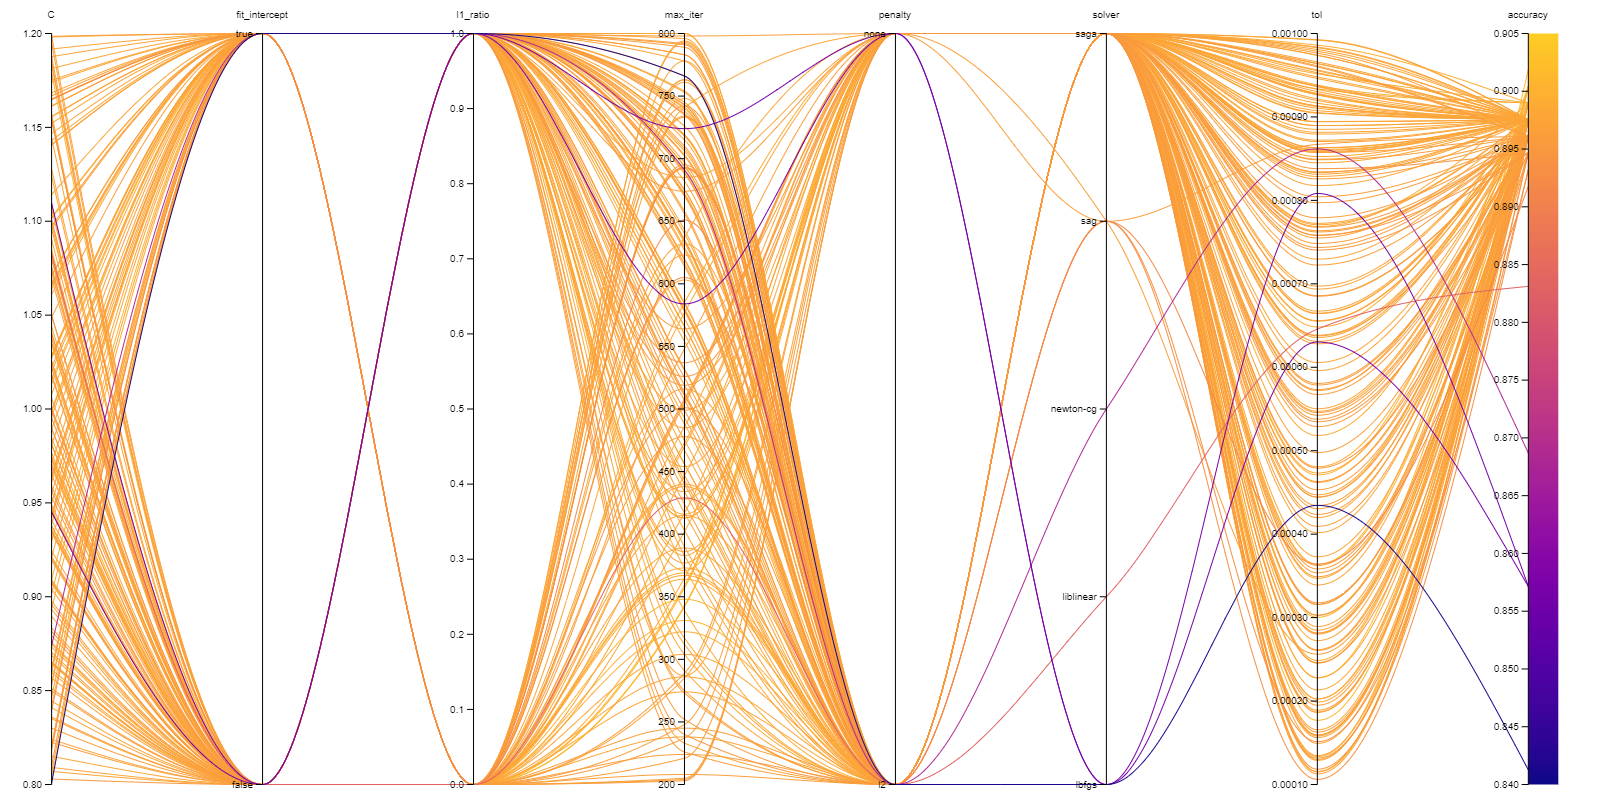
\includegraphics[width = \textwidth, height = \textwidth, keepaspectratio]{Images/LC ParallelCoordGraph.png}
\end{figure}

  \FloatBarrier
% =================== Multilayer Perceptron APPENDIX here ===================
\newpage
\section{Multilayer Perceptron}

\subsection{Multilayer Perceptron Parameter Importance}
  \begin{table}[ht]
    \centering
    \begin{tabular}{|p{0.3\linewidth} | p{0.3\linewidth}| p{0.3\linewidth}|} 
      \hline
      \textbf{Parameter Config}  & \textbf{Importance} & \textbf{Correlation} \\ \hline
        hidden\_layer\_sizes & 0.095 & -0.101 \\ \hline
        max\_iter & 0.091 & 0.072 \\ \hline
        alpha & 0.061 & 0.171 \\ \hline
    \end{tabular}
  \end{table}\label{MLP_ParamImp1}

  
  \begin{table}[ht]
    \centering
    \begin{tabular}{|p{0.3\linewidth} | p{0.3\linewidth}| p{0.3\linewidth}|} 
      \hline
      \textbf{Parameter Config}  & \textbf{Importance} & \textbf{Correlation} \\ \hline
        solver.value\_lbfgs & 0.530 & 0.728 \\ \hline
        solver.value\_adam & 0.027 & -0.245 \\ \hline
        solver.value\_sgd & 0.024 & -0.640 \\ \hline
        activation.value\_identity & 0.098 & -0.169 \\ \hline
        activation.value\_relu & 0.033 & 0.301 \\ \hline
        activation.value\_tanh & 0.018 & -0.035 \\ \hline
        activation.value\_logistic & 0.006 & -0.270 \\ \hline
        learning\_rate.value\_adaptive & 0.012 & 0.507 \\ \hline
        learning\_rate.value\_constant & 0.004 & -0.442 \\ \hline
        learning\_rate.value\_invscaling & 0.001 & -0.224 \\ \hline
    \end{tabular}
  \end{table}\label{MLP_ParamImp2}

\begin{figure}[h]
  \caption {Multilayer Perceptron Parameters} \label{ParallelCoordMLP}
  \centering 
  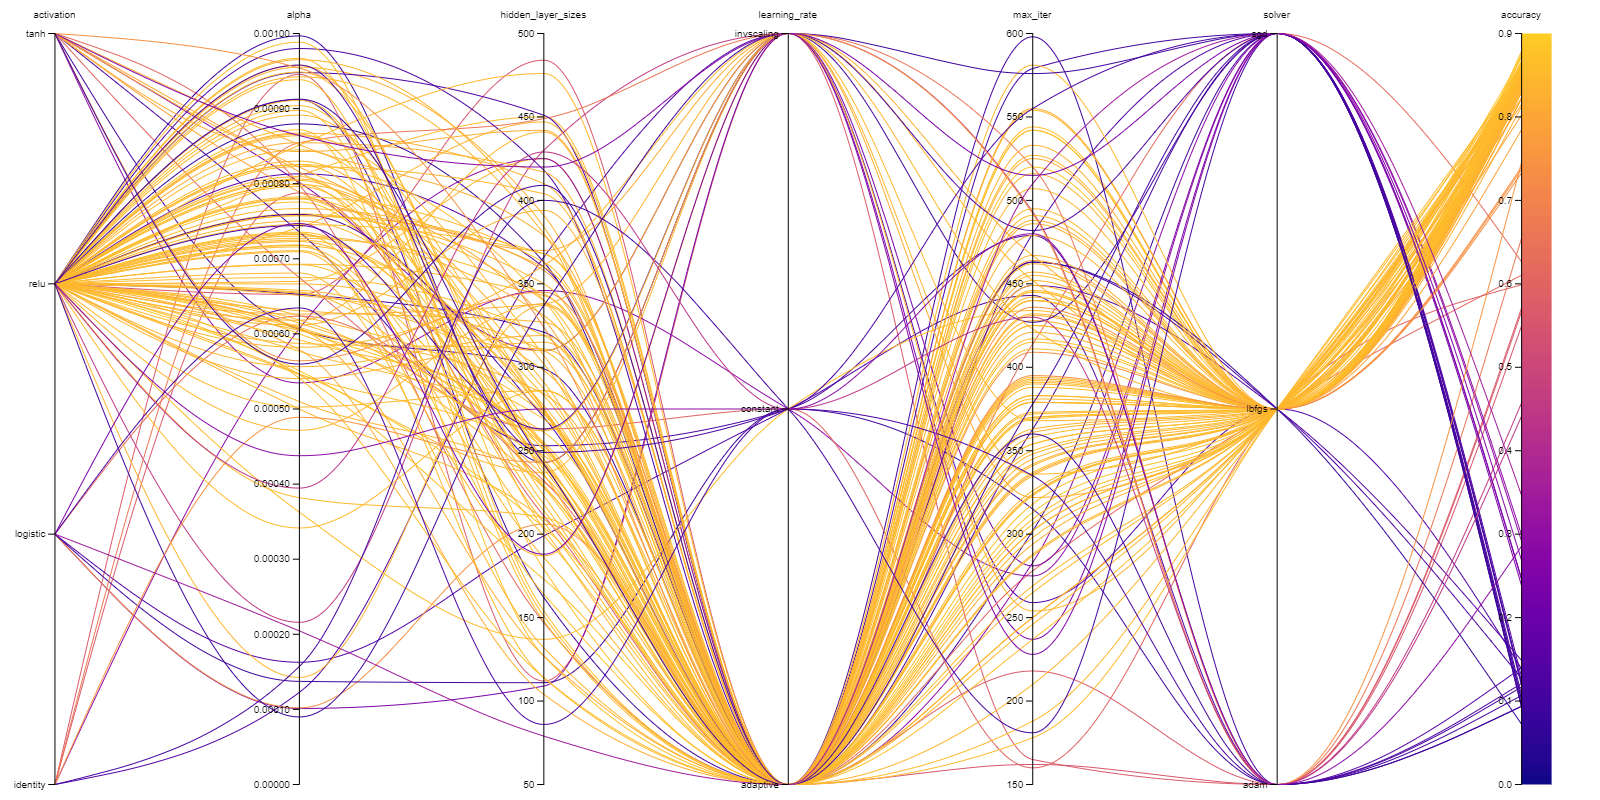
\includegraphics[width = \textwidth, height = \textwidth, keepaspectratio]{Images/MLP ParallelCoordGraph.png}
\end{figure}

\section{R41} \label{R41}
\url{https://scikit-learn.org/stable/modules/generated/sklearn.linear_model.LogisticRegression.html}

\FloatBarrier
% =================== END APPENDIX ===================
\end{appendices}

\newpage
\raggedright
\nocite{zhaoComparisonDecisionTree2008}
\bibliography{Library}
\bibliographystyle{plain}

\end{document}

  % \begin{sidewaysfigure}[h]
  %   \caption {Accuracy over time - J48} \label{J48AccOverTime}
  %   \centering
  %   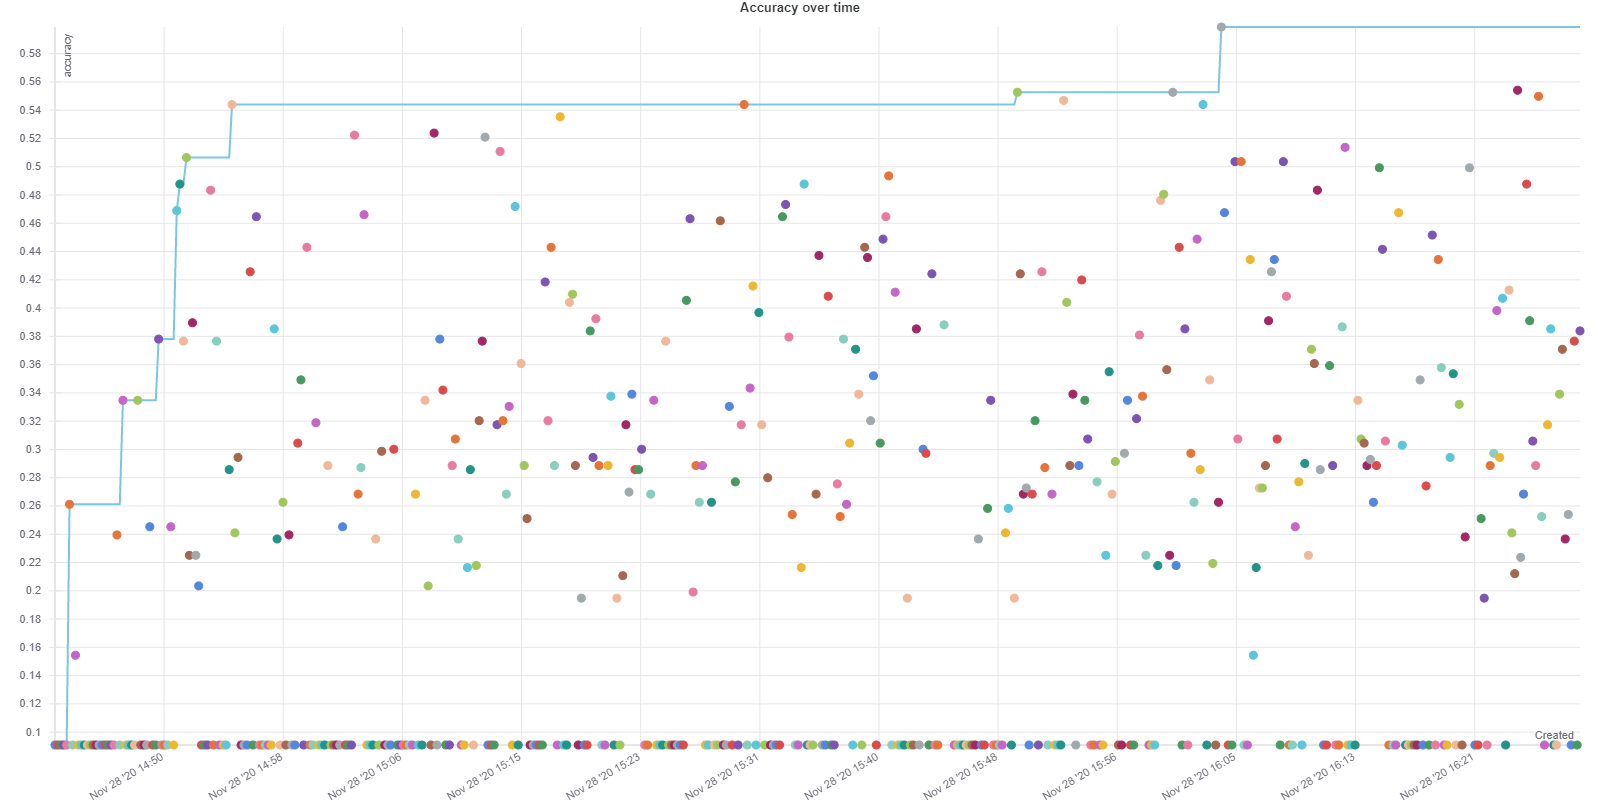
\includegraphics[width = \textwidth, height = \textwidth, keepaspectratio]{Images/J48 Acc over time.png}
  % \end{sidewaysfigure}